\documentclass[11pt]{article}

    \usepackage[breakable]{tcolorbox}
    \usepackage{parskip} % Stop auto-indenting (to mimic markdown behaviour)
    
    \usepackage{iftex}
    \ifPDFTeX
    	\usepackage[T1]{fontenc}
    	\usepackage{mathpazo}
    \else
    	\usepackage{fontspec}
    \fi

    % Basic figure setup, for now with no caption control since it's done
    % automatically by Pandoc (which extracts ![](path) syntax from Markdown).
    \usepackage{graphicx}
    % Maintain compatibility with old templates. Remove in nbconvert 6.0
    \let\Oldincludegraphics\includegraphics
    % Ensure that by default, figures have no caption (until we provide a
    % proper Figure object with a Caption API and a way to capture that
    % in the conversion process - todo).
    \usepackage{caption}
    \DeclareCaptionFormat{nocaption}{}
    \captionsetup{format=nocaption,aboveskip=0pt,belowskip=0pt}

    \usepackage[Export]{adjustbox} % Used to constrain images to a maximum size
    \adjustboxset{max size={0.9\linewidth}{0.9\paperheight}}
    \usepackage{float}
    \floatplacement{figure}{H} % forces figures to be placed at the correct location
    \usepackage{xcolor} % Allow colors to be defined
    \usepackage{enumerate} % Needed for markdown enumerations to work
    \usepackage{geometry} % Used to adjust the document margins
    \usepackage{amsmath} % Equations
    \usepackage{amssymb} % Equations
    \usepackage{textcomp} % defines textquotesingle
    % Hack from http://tex.stackexchange.com/a/47451/13684:
    \AtBeginDocument{%
        \def\PYZsq{\textquotesingle}% Upright quotes in Pygmentized code
    }
    \usepackage{upquote} % Upright quotes for verbatim code
    \usepackage{eurosym} % defines \euro
    \usepackage[mathletters]{ucs} % Extended unicode (utf-8) support
    \usepackage{fancyvrb} % verbatim replacement that allows latex
    \usepackage{grffile} % extends the file name processing of package graphics 
                         % to support a larger range
    \makeatletter % fix for grffile with XeLaTeX
    \def\Gread@@xetex#1{%
      \IfFileExists{"\Gin@base".bb}%
      {\Gread@eps{\Gin@base.bb}}%
      {\Gread@@xetex@aux#1}%
    }
    \makeatother

    % The hyperref package gives us a pdf with properly built
    % internal navigation ('pdf bookmarks' for the table of contents,
    % internal cross-reference links, web links for URLs, etc.)
    \usepackage{hyperref}
    % The default LaTeX title has an obnoxious amount of whitespace. By default,
    % titling removes some of it. It also provides customization options.
    \usepackage{titling}
    \usepackage{longtable} % longtable support required by pandoc >1.10
    \usepackage{booktabs}  % table support for pandoc > 1.12.2
    \usepackage[inline]{enumitem} % IRkernel/repr support (it uses the enumerate* environment)
    \usepackage[normalem]{ulem} % ulem is needed to support strikethroughs (\sout)
                                % normalem makes italics be italics, not underlines
    \usepackage{mathrsfs}
    

    
    % Colors for the hyperref package
    \definecolor{urlcolor}{rgb}{0,.145,.698}
    \definecolor{linkcolor}{rgb}{.71,0.21,0.01}
    \definecolor{citecolor}{rgb}{.12,.54,.11}

    % ANSI colors
    \definecolor{ansi-black}{HTML}{3E424D}
    \definecolor{ansi-black-intense}{HTML}{282C36}
    \definecolor{ansi-red}{HTML}{E75C58}
    \definecolor{ansi-red-intense}{HTML}{B22B31}
    \definecolor{ansi-green}{HTML}{00A250}
    \definecolor{ansi-green-intense}{HTML}{007427}
    \definecolor{ansi-yellow}{HTML}{DDB62B}
    \definecolor{ansi-yellow-intense}{HTML}{B27D12}
    \definecolor{ansi-blue}{HTML}{208FFB}
    \definecolor{ansi-blue-intense}{HTML}{0065CA}
    \definecolor{ansi-magenta}{HTML}{D160C4}
    \definecolor{ansi-magenta-intense}{HTML}{A03196}
    \definecolor{ansi-cyan}{HTML}{60C6C8}
    \definecolor{ansi-cyan-intense}{HTML}{258F8F}
    \definecolor{ansi-white}{HTML}{C5C1B4}
    \definecolor{ansi-white-intense}{HTML}{A1A6B2}
    \definecolor{ansi-default-inverse-fg}{HTML}{FFFFFF}
    \definecolor{ansi-default-inverse-bg}{HTML}{000000}

    % commands and environments needed by pandoc snippets
    % extracted from the output of `pandoc -s`
    \providecommand{\tightlist}{%
      \setlength{\itemsep}{0pt}\setlength{\parskip}{0pt}}
    \DefineVerbatimEnvironment{Highlighting}{Verbatim}{commandchars=\\\{\}}
    % Add ',fontsize=\small' for more characters per line
    \newenvironment{Shaded}{}{}
    \newcommand{\KeywordTok}[1]{\textcolor[rgb]{0.00,0.44,0.13}{\textbf{{#1}}}}
    \newcommand{\DataTypeTok}[1]{\textcolor[rgb]{0.56,0.13,0.00}{{#1}}}
    \newcommand{\DecValTok}[1]{\textcolor[rgb]{0.25,0.63,0.44}{{#1}}}
    \newcommand{\BaseNTok}[1]{\textcolor[rgb]{0.25,0.63,0.44}{{#1}}}
    \newcommand{\FloatTok}[1]{\textcolor[rgb]{0.25,0.63,0.44}{{#1}}}
    \newcommand{\CharTok}[1]{\textcolor[rgb]{0.25,0.44,0.63}{{#1}}}
    \newcommand{\StringTok}[1]{\textcolor[rgb]{0.25,0.44,0.63}{{#1}}}
    \newcommand{\CommentTok}[1]{\textcolor[rgb]{0.38,0.63,0.69}{\textit{{#1}}}}
    \newcommand{\OtherTok}[1]{\textcolor[rgb]{0.00,0.44,0.13}{{#1}}}
    \newcommand{\AlertTok}[1]{\textcolor[rgb]{1.00,0.00,0.00}{\textbf{{#1}}}}
    \newcommand{\FunctionTok}[1]{\textcolor[rgb]{0.02,0.16,0.49}{{#1}}}
    \newcommand{\RegionMarkerTok}[1]{{#1}}
    \newcommand{\ErrorTok}[1]{\textcolor[rgb]{1.00,0.00,0.00}{\textbf{{#1}}}}
    \newcommand{\NormalTok}[1]{{#1}}
    
    % Additional commands for more recent versions of Pandoc
    \newcommand{\ConstantTok}[1]{\textcolor[rgb]{0.53,0.00,0.00}{{#1}}}
    \newcommand{\SpecialCharTok}[1]{\textcolor[rgb]{0.25,0.44,0.63}{{#1}}}
    \newcommand{\VerbatimStringTok}[1]{\textcolor[rgb]{0.25,0.44,0.63}{{#1}}}
    \newcommand{\SpecialStringTok}[1]{\textcolor[rgb]{0.73,0.40,0.53}{{#1}}}
    \newcommand{\ImportTok}[1]{{#1}}
    \newcommand{\DocumentationTok}[1]{\textcolor[rgb]{0.73,0.13,0.13}{\textit{{#1}}}}
    \newcommand{\AnnotationTok}[1]{\textcolor[rgb]{0.38,0.63,0.69}{\textbf{\textit{{#1}}}}}
    \newcommand{\CommentVarTok}[1]{\textcolor[rgb]{0.38,0.63,0.69}{\textbf{\textit{{#1}}}}}
    \newcommand{\VariableTok}[1]{\textcolor[rgb]{0.10,0.09,0.49}{{#1}}}
    \newcommand{\ControlFlowTok}[1]{\textcolor[rgb]{0.00,0.44,0.13}{\textbf{{#1}}}}
    \newcommand{\OperatorTok}[1]{\textcolor[rgb]{0.40,0.40,0.40}{{#1}}}
    \newcommand{\BuiltInTok}[1]{{#1}}
    \newcommand{\ExtensionTok}[1]{{#1}}
    \newcommand{\PreprocessorTok}[1]{\textcolor[rgb]{0.74,0.48,0.00}{{#1}}}
    \newcommand{\AttributeTok}[1]{\textcolor[rgb]{0.49,0.56,0.16}{{#1}}}
    \newcommand{\InformationTok}[1]{\textcolor[rgb]{0.38,0.63,0.69}{\textbf{\textit{{#1}}}}}
    \newcommand{\WarningTok}[1]{\textcolor[rgb]{0.38,0.63,0.69}{\textbf{\textit{{#1}}}}}
    
    
    % Define a nice break command that doesn't care if a line doesn't already
    % exist.
    \def\br{\hspace*{\fill} \\* }
    % Math Jax compatibility definitions
    \def\gt{>}
    \def\lt{<}
    \let\Oldtex\TeX
    \let\Oldlatex\LaTeX
    \renewcommand{\TeX}{\textrm{\Oldtex}}
    \renewcommand{\LaTeX}{\textrm{\Oldlatex}}
    % Document parameters
    % Document title
    \title{fdaf}
    
    
    
    
    
% Pygments definitions
\makeatletter
\def\PY@reset{\let\PY@it=\relax \let\PY@bf=\relax%
    \let\PY@ul=\relax \let\PY@tc=\relax%
    \let\PY@bc=\relax \let\PY@ff=\relax}
\def\PY@tok#1{\csname PY@tok@#1\endcsname}
\def\PY@toks#1+{\ifx\relax#1\empty\else%
    \PY@tok{#1}\expandafter\PY@toks\fi}
\def\PY@do#1{\PY@bc{\PY@tc{\PY@ul{%
    \PY@it{\PY@bf{\PY@ff{#1}}}}}}}
\def\PY#1#2{\PY@reset\PY@toks#1+\relax+\PY@do{#2}}

\expandafter\def\csname PY@tok@w\endcsname{\def\PY@tc##1{\textcolor[rgb]{0.73,0.73,0.73}{##1}}}
\expandafter\def\csname PY@tok@c\endcsname{\let\PY@it=\textit\def\PY@tc##1{\textcolor[rgb]{0.25,0.50,0.50}{##1}}}
\expandafter\def\csname PY@tok@cp\endcsname{\def\PY@tc##1{\textcolor[rgb]{0.74,0.48,0.00}{##1}}}
\expandafter\def\csname PY@tok@k\endcsname{\let\PY@bf=\textbf\def\PY@tc##1{\textcolor[rgb]{0.00,0.50,0.00}{##1}}}
\expandafter\def\csname PY@tok@kp\endcsname{\def\PY@tc##1{\textcolor[rgb]{0.00,0.50,0.00}{##1}}}
\expandafter\def\csname PY@tok@kt\endcsname{\def\PY@tc##1{\textcolor[rgb]{0.69,0.00,0.25}{##1}}}
\expandafter\def\csname PY@tok@o\endcsname{\def\PY@tc##1{\textcolor[rgb]{0.40,0.40,0.40}{##1}}}
\expandafter\def\csname PY@tok@ow\endcsname{\let\PY@bf=\textbf\def\PY@tc##1{\textcolor[rgb]{0.67,0.13,1.00}{##1}}}
\expandafter\def\csname PY@tok@nb\endcsname{\def\PY@tc##1{\textcolor[rgb]{0.00,0.50,0.00}{##1}}}
\expandafter\def\csname PY@tok@nf\endcsname{\def\PY@tc##1{\textcolor[rgb]{0.00,0.00,1.00}{##1}}}
\expandafter\def\csname PY@tok@nc\endcsname{\let\PY@bf=\textbf\def\PY@tc##1{\textcolor[rgb]{0.00,0.00,1.00}{##1}}}
\expandafter\def\csname PY@tok@nn\endcsname{\let\PY@bf=\textbf\def\PY@tc##1{\textcolor[rgb]{0.00,0.00,1.00}{##1}}}
\expandafter\def\csname PY@tok@ne\endcsname{\let\PY@bf=\textbf\def\PY@tc##1{\textcolor[rgb]{0.82,0.25,0.23}{##1}}}
\expandafter\def\csname PY@tok@nv\endcsname{\def\PY@tc##1{\textcolor[rgb]{0.10,0.09,0.49}{##1}}}
\expandafter\def\csname PY@tok@no\endcsname{\def\PY@tc##1{\textcolor[rgb]{0.53,0.00,0.00}{##1}}}
\expandafter\def\csname PY@tok@nl\endcsname{\def\PY@tc##1{\textcolor[rgb]{0.63,0.63,0.00}{##1}}}
\expandafter\def\csname PY@tok@ni\endcsname{\let\PY@bf=\textbf\def\PY@tc##1{\textcolor[rgb]{0.60,0.60,0.60}{##1}}}
\expandafter\def\csname PY@tok@na\endcsname{\def\PY@tc##1{\textcolor[rgb]{0.49,0.56,0.16}{##1}}}
\expandafter\def\csname PY@tok@nt\endcsname{\let\PY@bf=\textbf\def\PY@tc##1{\textcolor[rgb]{0.00,0.50,0.00}{##1}}}
\expandafter\def\csname PY@tok@nd\endcsname{\def\PY@tc##1{\textcolor[rgb]{0.67,0.13,1.00}{##1}}}
\expandafter\def\csname PY@tok@s\endcsname{\def\PY@tc##1{\textcolor[rgb]{0.73,0.13,0.13}{##1}}}
\expandafter\def\csname PY@tok@sd\endcsname{\let\PY@it=\textit\def\PY@tc##1{\textcolor[rgb]{0.73,0.13,0.13}{##1}}}
\expandafter\def\csname PY@tok@si\endcsname{\let\PY@bf=\textbf\def\PY@tc##1{\textcolor[rgb]{0.73,0.40,0.53}{##1}}}
\expandafter\def\csname PY@tok@se\endcsname{\let\PY@bf=\textbf\def\PY@tc##1{\textcolor[rgb]{0.73,0.40,0.13}{##1}}}
\expandafter\def\csname PY@tok@sr\endcsname{\def\PY@tc##1{\textcolor[rgb]{0.73,0.40,0.53}{##1}}}
\expandafter\def\csname PY@tok@ss\endcsname{\def\PY@tc##1{\textcolor[rgb]{0.10,0.09,0.49}{##1}}}
\expandafter\def\csname PY@tok@sx\endcsname{\def\PY@tc##1{\textcolor[rgb]{0.00,0.50,0.00}{##1}}}
\expandafter\def\csname PY@tok@m\endcsname{\def\PY@tc##1{\textcolor[rgb]{0.40,0.40,0.40}{##1}}}
\expandafter\def\csname PY@tok@gh\endcsname{\let\PY@bf=\textbf\def\PY@tc##1{\textcolor[rgb]{0.00,0.00,0.50}{##1}}}
\expandafter\def\csname PY@tok@gu\endcsname{\let\PY@bf=\textbf\def\PY@tc##1{\textcolor[rgb]{0.50,0.00,0.50}{##1}}}
\expandafter\def\csname PY@tok@gd\endcsname{\def\PY@tc##1{\textcolor[rgb]{0.63,0.00,0.00}{##1}}}
\expandafter\def\csname PY@tok@gi\endcsname{\def\PY@tc##1{\textcolor[rgb]{0.00,0.63,0.00}{##1}}}
\expandafter\def\csname PY@tok@gr\endcsname{\def\PY@tc##1{\textcolor[rgb]{1.00,0.00,0.00}{##1}}}
\expandafter\def\csname PY@tok@ge\endcsname{\let\PY@it=\textit}
\expandafter\def\csname PY@tok@gs\endcsname{\let\PY@bf=\textbf}
\expandafter\def\csname PY@tok@gp\endcsname{\let\PY@bf=\textbf\def\PY@tc##1{\textcolor[rgb]{0.00,0.00,0.50}{##1}}}
\expandafter\def\csname PY@tok@go\endcsname{\def\PY@tc##1{\textcolor[rgb]{0.53,0.53,0.53}{##1}}}
\expandafter\def\csname PY@tok@gt\endcsname{\def\PY@tc##1{\textcolor[rgb]{0.00,0.27,0.87}{##1}}}
\expandafter\def\csname PY@tok@err\endcsname{\def\PY@bc##1{\setlength{\fboxsep}{0pt}\fcolorbox[rgb]{1.00,0.00,0.00}{1,1,1}{\strut ##1}}}
\expandafter\def\csname PY@tok@kc\endcsname{\let\PY@bf=\textbf\def\PY@tc##1{\textcolor[rgb]{0.00,0.50,0.00}{##1}}}
\expandafter\def\csname PY@tok@kd\endcsname{\let\PY@bf=\textbf\def\PY@tc##1{\textcolor[rgb]{0.00,0.50,0.00}{##1}}}
\expandafter\def\csname PY@tok@kn\endcsname{\let\PY@bf=\textbf\def\PY@tc##1{\textcolor[rgb]{0.00,0.50,0.00}{##1}}}
\expandafter\def\csname PY@tok@kr\endcsname{\let\PY@bf=\textbf\def\PY@tc##1{\textcolor[rgb]{0.00,0.50,0.00}{##1}}}
\expandafter\def\csname PY@tok@bp\endcsname{\def\PY@tc##1{\textcolor[rgb]{0.00,0.50,0.00}{##1}}}
\expandafter\def\csname PY@tok@fm\endcsname{\def\PY@tc##1{\textcolor[rgb]{0.00,0.00,1.00}{##1}}}
\expandafter\def\csname PY@tok@vc\endcsname{\def\PY@tc##1{\textcolor[rgb]{0.10,0.09,0.49}{##1}}}
\expandafter\def\csname PY@tok@vg\endcsname{\def\PY@tc##1{\textcolor[rgb]{0.10,0.09,0.49}{##1}}}
\expandafter\def\csname PY@tok@vi\endcsname{\def\PY@tc##1{\textcolor[rgb]{0.10,0.09,0.49}{##1}}}
\expandafter\def\csname PY@tok@vm\endcsname{\def\PY@tc##1{\textcolor[rgb]{0.10,0.09,0.49}{##1}}}
\expandafter\def\csname PY@tok@sa\endcsname{\def\PY@tc##1{\textcolor[rgb]{0.73,0.13,0.13}{##1}}}
\expandafter\def\csname PY@tok@sb\endcsname{\def\PY@tc##1{\textcolor[rgb]{0.73,0.13,0.13}{##1}}}
\expandafter\def\csname PY@tok@sc\endcsname{\def\PY@tc##1{\textcolor[rgb]{0.73,0.13,0.13}{##1}}}
\expandafter\def\csname PY@tok@dl\endcsname{\def\PY@tc##1{\textcolor[rgb]{0.73,0.13,0.13}{##1}}}
\expandafter\def\csname PY@tok@s2\endcsname{\def\PY@tc##1{\textcolor[rgb]{0.73,0.13,0.13}{##1}}}
\expandafter\def\csname PY@tok@sh\endcsname{\def\PY@tc##1{\textcolor[rgb]{0.73,0.13,0.13}{##1}}}
\expandafter\def\csname PY@tok@s1\endcsname{\def\PY@tc##1{\textcolor[rgb]{0.73,0.13,0.13}{##1}}}
\expandafter\def\csname PY@tok@mb\endcsname{\def\PY@tc##1{\textcolor[rgb]{0.40,0.40,0.40}{##1}}}
\expandafter\def\csname PY@tok@mf\endcsname{\def\PY@tc##1{\textcolor[rgb]{0.40,0.40,0.40}{##1}}}
\expandafter\def\csname PY@tok@mh\endcsname{\def\PY@tc##1{\textcolor[rgb]{0.40,0.40,0.40}{##1}}}
\expandafter\def\csname PY@tok@mi\endcsname{\def\PY@tc##1{\textcolor[rgb]{0.40,0.40,0.40}{##1}}}
\expandafter\def\csname PY@tok@il\endcsname{\def\PY@tc##1{\textcolor[rgb]{0.40,0.40,0.40}{##1}}}
\expandafter\def\csname PY@tok@mo\endcsname{\def\PY@tc##1{\textcolor[rgb]{0.40,0.40,0.40}{##1}}}
\expandafter\def\csname PY@tok@ch\endcsname{\let\PY@it=\textit\def\PY@tc##1{\textcolor[rgb]{0.25,0.50,0.50}{##1}}}
\expandafter\def\csname PY@tok@cm\endcsname{\let\PY@it=\textit\def\PY@tc##1{\textcolor[rgb]{0.25,0.50,0.50}{##1}}}
\expandafter\def\csname PY@tok@cpf\endcsname{\let\PY@it=\textit\def\PY@tc##1{\textcolor[rgb]{0.25,0.50,0.50}{##1}}}
\expandafter\def\csname PY@tok@c1\endcsname{\let\PY@it=\textit\def\PY@tc##1{\textcolor[rgb]{0.25,0.50,0.50}{##1}}}
\expandafter\def\csname PY@tok@cs\endcsname{\let\PY@it=\textit\def\PY@tc##1{\textcolor[rgb]{0.25,0.50,0.50}{##1}}}

\def\PYZbs{\char`\\}
\def\PYZus{\char`\_}
\def\PYZob{\char`\{}
\def\PYZcb{\char`\}}
\def\PYZca{\char`\^}
\def\PYZam{\char`\&}
\def\PYZlt{\char`\<}
\def\PYZgt{\char`\>}
\def\PYZsh{\char`\#}
\def\PYZpc{\char`\%}
\def\PYZdl{\char`\$}
\def\PYZhy{\char`\-}
\def\PYZsq{\char`\'}
\def\PYZdq{\char`\"}
\def\PYZti{\char`\~}
% for compatibility with earlier versions
\def\PYZat{@}
\def\PYZlb{[}
\def\PYZrb{]}
\makeatother


    % For linebreaks inside Verbatim environment from package fancyvrb. 
    \makeatletter
        \newbox\Wrappedcontinuationbox 
        \newbox\Wrappedvisiblespacebox 
        \newcommand*\Wrappedvisiblespace {\textcolor{red}{\textvisiblespace}} 
        \newcommand*\Wrappedcontinuationsymbol {\textcolor{red}{\llap{\tiny$\m@th\hookrightarrow$}}} 
        \newcommand*\Wrappedcontinuationindent {3ex } 
        \newcommand*\Wrappedafterbreak {\kern\Wrappedcontinuationindent\copy\Wrappedcontinuationbox} 
        % Take advantage of the already applied Pygments mark-up to insert 
        % potential linebreaks for TeX processing. 
        %        {, <, #, %, $, ' and ": go to next line. 
        %        _, }, ^, &, >, - and ~: stay at end of broken line. 
        % Use of \textquotesingle for straight quote. 
        \newcommand*\Wrappedbreaksatspecials {% 
            \def\PYGZus{\discretionary{\char`\_}{\Wrappedafterbreak}{\char`\_}}% 
            \def\PYGZob{\discretionary{}{\Wrappedafterbreak\char`\{}{\char`\{}}% 
            \def\PYGZcb{\discretionary{\char`\}}{\Wrappedafterbreak}{\char`\}}}% 
            \def\PYGZca{\discretionary{\char`\^}{\Wrappedafterbreak}{\char`\^}}% 
            \def\PYGZam{\discretionary{\char`\&}{\Wrappedafterbreak}{\char`\&}}% 
            \def\PYGZlt{\discretionary{}{\Wrappedafterbreak\char`\<}{\char`\<}}% 
            \def\PYGZgt{\discretionary{\char`\>}{\Wrappedafterbreak}{\char`\>}}% 
            \def\PYGZsh{\discretionary{}{\Wrappedafterbreak\char`\#}{\char`\#}}% 
            \def\PYGZpc{\discretionary{}{\Wrappedafterbreak\char`\%}{\char`\%}}% 
            \def\PYGZdl{\discretionary{}{\Wrappedafterbreak\char`\$}{\char`\$}}% 
            \def\PYGZhy{\discretionary{\char`\-}{\Wrappedafterbreak}{\char`\-}}% 
            \def\PYGZsq{\discretionary{}{\Wrappedafterbreak\textquotesingle}{\textquotesingle}}% 
            \def\PYGZdq{\discretionary{}{\Wrappedafterbreak\char`\"}{\char`\"}}% 
            \def\PYGZti{\discretionary{\char`\~}{\Wrappedafterbreak}{\char`\~}}% 
        } 
        % Some characters . , ; ? ! / are not pygmentized. 
        % This macro makes them "active" and they will insert potential linebreaks 
        \newcommand*\Wrappedbreaksatpunct {% 
            \lccode`\~`\.\lowercase{\def~}{\discretionary{\hbox{\char`\.}}{\Wrappedafterbreak}{\hbox{\char`\.}}}% 
            \lccode`\~`\,\lowercase{\def~}{\discretionary{\hbox{\char`\,}}{\Wrappedafterbreak}{\hbox{\char`\,}}}% 
            \lccode`\~`\;\lowercase{\def~}{\discretionary{\hbox{\char`\;}}{\Wrappedafterbreak}{\hbox{\char`\;}}}% 
            \lccode`\~`\:\lowercase{\def~}{\discretionary{\hbox{\char`\:}}{\Wrappedafterbreak}{\hbox{\char`\:}}}% 
            \lccode`\~`\?\lowercase{\def~}{\discretionary{\hbox{\char`\?}}{\Wrappedafterbreak}{\hbox{\char`\?}}}% 
            \lccode`\~`\!\lowercase{\def~}{\discretionary{\hbox{\char`\!}}{\Wrappedafterbreak}{\hbox{\char`\!}}}% 
            \lccode`\~`\/\lowercase{\def~}{\discretionary{\hbox{\char`\/}}{\Wrappedafterbreak}{\hbox{\char`\/}}}% 
            \catcode`\.\active
            \catcode`\,\active 
            \catcode`\;\active
            \catcode`\:\active
            \catcode`\?\active
            \catcode`\!\active
            \catcode`\/\active 
            \lccode`\~`\~ 	
        }
    \makeatother

    \let\OriginalVerbatim=\Verbatim
    \makeatletter
    \renewcommand{\Verbatim}[1][1]{%
        %\parskip\z@skip
        \sbox\Wrappedcontinuationbox {\Wrappedcontinuationsymbol}%
        \sbox\Wrappedvisiblespacebox {\FV@SetupFont\Wrappedvisiblespace}%
        \def\FancyVerbFormatLine ##1{\hsize\linewidth
            \vtop{\raggedright\hyphenpenalty\z@\exhyphenpenalty\z@
                \doublehyphendemerits\z@\finalhyphendemerits\z@
                \strut ##1\strut}%
        }%
        % If the linebreak is at a space, the latter will be displayed as visible
        % space at end of first line, and a continuation symbol starts next line.
        % Stretch/shrink are however usually zero for typewriter font.
        \def\FV@Space {%
            \nobreak\hskip\z@ plus\fontdimen3\font minus\fontdimen4\font
            \discretionary{\copy\Wrappedvisiblespacebox}{\Wrappedafterbreak}
            {\kern\fontdimen2\font}%
        }%
        
        % Allow breaks at special characters using \PYG... macros.
        \Wrappedbreaksatspecials
        % Breaks at punctuation characters . , ; ? ! and / need catcode=\active 	
        \OriginalVerbatim[#1,codes*=\Wrappedbreaksatpunct]%
    }
    \makeatother

    % Exact colors from NB
    \definecolor{incolor}{HTML}{303F9F}
    \definecolor{outcolor}{HTML}{D84315}
    \definecolor{cellborder}{HTML}{CFCFCF}
    \definecolor{cellbackground}{HTML}{F7F7F7}
    
    % prompt
    \makeatletter
    \newcommand{\boxspacing}{\kern\kvtcb@left@rule\kern\kvtcb@boxsep}
    \makeatother
    \newcommand{\prompt}[4]{
        \ttfamily\llap{{\color{#2}[#3]:\hspace{3pt}#4}}\vspace{-\baselineskip}
    }
    

    
    % Prevent overflowing lines due to hard-to-break entities
    \sloppy 
    % Setup hyperref package
    \hypersetup{
      breaklinks=true,  % so long urls are correctly broken across lines
      colorlinks=true,
      urlcolor=urlcolor,
      linkcolor=linkcolor,
      citecolor=citecolor,
      }
    % Slightly bigger margins than the latex defaults
    
    \geometry{verbose,tmargin=1in,bmargin=1in,lmargin=1in,rmargin=1in}
    
    

\begin{document}
    
    \maketitle
    
    

    
    \hypertarget{frequency-domain-adaptive-filtering-for-acoustic-echo-cancellation}{%
\section{Frequency Domain Adaptive Filtering for Acoustic Echo
Cancellation}\label{frequency-domain-adaptive-filtering-for-acoustic-echo-cancellation}}

\textbf{Prepared by} \textbar{} Unal Ege Gaznepoglu \& Jan Wilczek
\textbf{Matrikel Nr} \textbar{} 22746880 \& 22736060 \textbf{E-mail
Addr} \textbar{} ege.gaznepoglu@fau.de \& jan.wilczek@fau.de

    \hypertarget{introduction-motivation}{%
\subsection{1. Introduction \&
Motivation}\label{introduction-motivation}}

Acoustic Echo Cancellation (AEC) is a long-worked problem for which many
algorithms have been developed. The visual below illustrates the
problem:

\begin{figure}
\centering
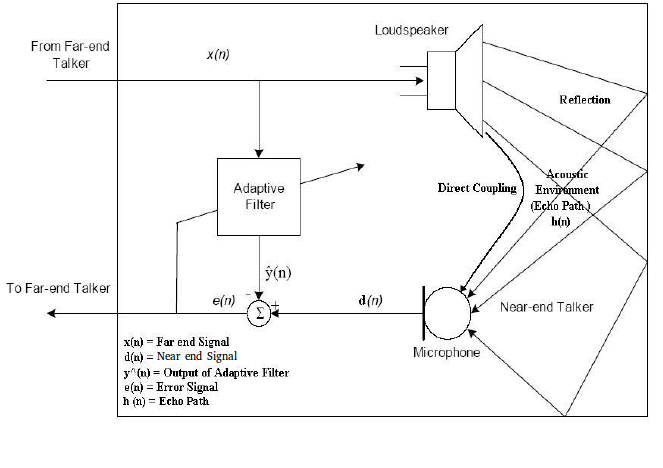
\includegraphics{./Images/Fig1-AECdesc.png}
\caption{Figure 1: Acoustic Echo Cancellation problem description}
\end{figure}

Given \(x(n)\) and \(d(n)\), we wish to extract \(e(n)\). This is
possible with an adaptive filter \(\hat{h}(n)\) which should replicate
the actual environment's impulse response \(h(n)\). Ignoring any
non-linearities, there are various algorithms which solve the problem,
one being Least Mean-Squares (LMS). LMS is a time-domain algorithm and
we have realized its implementation during the 5th PrStaSip laboratory
session. Variations include the block-LMS algorithm which updates the
filter coefficients once per block of new samples instead of every
sample.

However, a drawback of LMS is the fast-growing complexity with the
impulse response length. The fast Fourier transform allows more
efficient filtering in frequency domain, so a frequency-domain
complement - Frequency Domain Adaptive Filtering (FDAF) has been
described by Shynk {[}1{]}.

With the adaptive algorithms, a new problem emerges: when one should
`adapt' the filter and when one should not. From our experience in
related PrStaSiP session, we discovered that adaptation during
double-talk (both far-end and near-end speakers active at the same time)
severely degrades the algorithm's performance. This is to be expected as
during double-talk the \(e(n)\) has two components: one resulting from
inadequate adaptation filter's estimate and the other coming from the
near-end speaker. The latter carries no information regarding \(h(n)\),
yet affects the update. To summarize, we have to stop adaptation
whenever we detect double-talk.

In laboratory session, for this purpose, we used a parameter called
\texttt{freeze\_index}, which stops the adaptation after a fixed number
of samples. As it is impossible to know ahead when precisely adaptation
should be put on hold during real-time filtering (e.g.~while performing
hands-free communication) a separate algorithm for detecting double-talk
must be implemented. For this purpose, we have chosen a double-talk
detector (DTD) using excitation-weighted mean magnitude square coherence
based on {[}3{]}.

    \hypertarget{notation}{%
\subsection{2. Notation}\label{notation}}

\hypertarget{vectors-matrices-scalars}{%
\subsubsection{2.1 Vectors, Matrices,
Scalars}\label{vectors-matrices-scalars}}

\$ F\_N :\$ FFT matrix of size (N x N)

\$ \{x\} :\$ Time domain vector

\$ \{A\} :\$ Time domain matrix

\$ \mathbf{x} :\$ Frequency domain vector

\$ \mathbf{A} :\$ Frequency domain matrix

\hypertarget{operators}{%
\subsubsection{2.2 Operators}\label{operators}}

\$ * \$ : convolution

\$ \odot \$ : elementwise product (Hadamard product)

\hypertarget{symbol-definitions}{%
\subsubsection{2.3 Symbol Definitions}\label{symbol-definitions}}

\begin{longtable}[]{@{}lll@{}}
\toprule
Desc. & Time-Domain & Frequency-Domain\tabularnewline
\midrule
\endhead
Filter coefficients & \(h(n)\) & \(\mathbf{h}(n)\)\tabularnewline
Loudspeaker signal & \(x(n)\) & \(\mathbf{x}(n)\),
\(\mathbf{X}(n)\)\tabularnewline
Microphone signal & \(d(n)\) & \(\mathbf{d}(n)\)\tabularnewline
Filter output & \(y(n)\) & \(\mathbf{y}(n)\)\tabularnewline
Error signal & \(e(n)\) & \(\mathbf{e}(n)\)\tabularnewline
PSD estimate & N/A & \(\mathbf{p_x}(n)\)\tabularnewline
Learning rate & N/A & \(\mathbf{M}(n)\)\tabularnewline
\bottomrule
\end{longtable}

For notational convenience (to be able to use matrix products all the
time), we denote \(\mathbf{X}(n)\) as frequency domain diagonal matrix
with elements of \(\mathbf{x}(n)\) on the main diagonal.

\begin{longtable}[]{@{}lll@{}}
\toprule
\begin{minipage}[b]{0.30\columnwidth}\raggedright
Symbol\strut
\end{minipage} & \begin{minipage}[b]{0.30\columnwidth}\raggedright
Definition\strut
\end{minipage} & \begin{minipage}[b]{0.30\columnwidth}\raggedright
Desc\strut
\end{minipage}\tabularnewline
\midrule
\endhead
\begin{minipage}[t]{0.30\columnwidth}\raggedright
\(G_{2N \times 2N}\)\strut
\end{minipage} & \begin{minipage}[t]{0.30\columnwidth}\raggedright
\(\begin{bmatrix} I_N & 0\\ 0 & 0 \end{bmatrix}\)\strut
\end{minipage} & \begin{minipage}[t]{0.30\columnwidth}\raggedright
Gradient constraint \#1\strut
\end{minipage}\tabularnewline
\begin{minipage}[t]{0.30\columnwidth}\raggedright
\(K_{N \times 2N}\)\strut
\end{minipage} & \begin{minipage}[t]{0.30\columnwidth}\raggedright
\(\begin{bmatrix} 0 & I_N\end{bmatrix}\)\strut
\end{minipage} & \begin{minipage}[t]{0.30\columnwidth}\raggedright
Gradient constraint \#2\strut
\end{minipage}\tabularnewline
\bottomrule
\end{longtable}

\hypertarget{parameters}{%
\subsubsection{2.4 Parameters}\label{parameters}}

\begin{longtable}[]{@{}ll@{}}
\toprule
Symbol & Desc.\tabularnewline
\midrule
\endhead
Block length & \(2N\)\tabularnewline
Shift count & \(N\)\tabularnewline
PSD leak factor & \(\lambda\)\tabularnewline
Learning rate multiplier & \(\mu\)\tabularnewline
PSD leak factor for coherence calculation & \(\lambda_c\)\tabularnewline
Double-talk detection threshold (open-loop) & \(T_{ol}\)\tabularnewline
Double-talk detection threshold (closed-loop) &
\(T_{cl}\)\tabularnewline
\bottomrule
\end{longtable}

    \hypertarget{lms-fdaf-and-emcd---theory}{%
\subsection{2. LMS, FDAF and EMCD -
Theory}\label{lms-fdaf-and-emcd---theory}}

\hypertarget{lms}{%
\subsubsection{2.1 LMS}\label{lms}}

All the LMS variants (block and non-block - time domain) try to minimize
the MSE.

\$ \zeta = E{[}e\^{}2(n){]}\$, where \(e(n) = d(n) - \hat{h}(h)*x(n)\)
(for convenience one can define \(y(n) = \hat{h}(n) * x(n)\))

To minimize MSE, LMS uses the following update rule (learning rule):
\(h_{n+1}(n) = h_{n}(n) + 2\mu e(n)x(n)\) and block-LMS uses the block
version :
\(h_{n+L}(n) = h_{n}(n) + \sum_{i=1}^{L} 2\mu e(n-L+i)x(n-L+i)\).
\(\mu\) is the learning rate, which could be picked to be a scalar
(vanilla) or a vector (e.g.~normalized LMS).

\hypertarget{fdaf}{%
\subsubsection{2.2 FDAF}\label{fdaf}}

Main characteristic of FDAF is that it features fast convolution in
frequency domain. Instead of performing \(x(n) * h(n)\), for FDAF we do
\(\mathbf{Y = \mathbf{h} \odot \mathbf{x}}\). To replicate the Hadamard
product using matrix operations, we store \(\mathbf{x}\) as a diagonal
matrix \(\mathbf{X}\) as discussed in the notation section.

An unavoidable result of frequency domain filtering is the circular
convolution effect. To avoid this, one should use the gradient
constraints: for the filtering operation as above, only the last \(N\)
elements (in the time-domain) should be non-zero, rest should be zero.
Multiplication with matrices \(G\) and \(K\) enforces that constraint.

Please note that out of various implementation possibilities, we decided
to go with overlap-and-save variant. The algorithm's steps are as
follows:

\hypertarget{initialize-only-once-at-the-beginning}{%
\paragraph{1. Initialize (only once at the
beginning)}\label{initialize-only-once-at-the-beginning}}

\begin{itemize}
\tightlist
\item
  Begin with an all-zeros filter.
\item
  Begin with a prior PSD estimate (if there is none, just set 0 or some
  small constant)
\end{itemize}

\hypertarget{per-block}{%
\paragraph{2. Per block:}\label{per-block}}

\hypertarget{compute-mathbfyn-and-mathbfen}{%
\subparagraph{\texorpdfstring{2.1 Compute \(\mathbf{y}(n)\) and
\(\mathbf{E}(n)\)}{2.1 Compute \textbackslash{}mathbf\{y\}(n) and \textbackslash{}mathbf\{E\}(n)}}\label{compute-mathbfyn-and-mathbfen}}

\begin{itemize}
\tightlist
\item
  \(\mathbf{y}(n) = K F^{-1} \mathbf{X}(n) \mathbf{h}(n)\)
\item
  \(\mathbf{e}(n) = \mathbf{d}(n) - \mathbf{y}(n)\)
\item
  \(\mathbf{E}(n) = F K^{T} \mathbf{e}(n)\)
\end{itemize}

\hypertarget{estimate-psd-of-x-then-compute-normalized-learning-rate}{%
\subparagraph{2.2 Estimate PSD of X, then compute normalized learning
rate}\label{estimate-psd-of-x-then-compute-normalized-learning-rate}}

\begin{itemize}
\tightlist
\item
  \$\mathbf{p}\_x(n) = \lambda \mathbf{p}\_x(n-1) + (1 - \lambda)
  X\^{}H(n) X(n) \$
\item
  \(\mathbf{M}(n) = \mu \, diag(\mathbf{p}_x(n)^{-1})\) (elementwise
  reciprocal)
\end{itemize}

\hypertarget{update-weight-vector}{%
\subparagraph{2.3 Update weight vector}\label{update-weight-vector}}

\begin{itemize}
\tightlist
\item
  \(\mathbf{h}(n) = \mathbf{h}(n-1) + 2 F G F^{-1} M(n) X^H(n)E(n)\)
\end{itemize}

\hypertarget{excitation-weighted-mean-magnitude-square-coherence-based-double-talk-detector}{%
\subsubsection{2.3 Excitation-weighted mean magnitude square
coherence-based double-talk
detector}\label{excitation-weighted-mean-magnitude-square-coherence-based-double-talk-detector}}

While initial propositions regarding double-talk detection incorporated
time-domain correlation calculation and comparison, modern approaches
turn to frequency-domain coherence {[}2{]}. The key point is to
formulate a decision variable \(\xi\), which can be then compared
against some threshold \(T\) in order to determine whether double-talk
was present in the block of samples {[}3{]}. For that we need the
estimates of auto- and cross- power spectral densities (PSDs) calculated
on a block-by-block basis:

\(\mathbf{s_{xx}}(n) = \lambda_c \mathbf{s_{xx}}(n-1) + (1 - \lambda_c) |\mathbf{x}(n)|^2\)

\(\mathbf{s_{dd}}(n) = \lambda_c \mathbf{s_{dd}}(n-1) + (1 - \lambda_c) |\mathbf{d}(n)|^2\)

\(\mathbf{s_{\hat{y}\hat{y}}}(n) = \lambda_c \mathbf{s_{\hat{y}\hat{y}}}(n-1) + (1 - \lambda_c) |\mathbf{\hat{y}}(n)|^2\)

\$\mathbf{s_{xd}}(n) = \lambda\_c \mathbf{s_{xd}}(n-1) + (1 -
\lambda\_c) \mathbf{x}(n) \odot \mathbf{d}(n)\^{}* \$

\$\mathbf{s_{\hat{y}d}}(n) = \lambda\_c \mathbf{s_{\hat{y}d}}(n-1) + (1
- \lambda\_c) \mathbf{\hat{y}}(n) \odot \mathbf{d}(n)\^{}* \$

where \(\lambda_c\) denotes PSD leak factor for coherence calculation
purposes, \(| \cdot |^2\) denotes element-wise squared absolute value,
and \(\cdot^*\) denotes element-wise complex conjugate.

The \(\xi\) variable incorporates weighted average of appropriate PSDs
ratios. We differentiate between two cases {[}4{]}: 1. Open-loop
structure: we take delayed version of the loudspeaker signal and compare
it to the microphone signal. Then the so-called coherence function reads

\(\gamma_{xd} = \frac{|\mathbf{s_{xd}}(n)|^2}{\mathbf{s_{xx}}(n) \odot \mathbf{s_{dd}}(n)}\)

and the \(\xi\) decision variable is equal to

\(\xi_{ol} = \sum_{f} \frac{\mathbf{s_{xx}}(n)}{\sum_{f}\mathbf{s_{xx}}(n)} \odot \gamma_{xd}\)

where \(ol\) subscript stands for `open-loop' and summation is always
over frequency bins. 2. Closed-loop structure: we take the output of the
adaptive filter and compare it to the microphone signal. Then the
coherence function reads:

\(\gamma_{\hat{y}d} = \frac{|\mathbf{s_{\hat{y}d}}(n)|^2}{\mathbf{s_{\hat{y}\hat{y}}}(n) \odot \mathbf{s_{dd}}(n)}\)

and the \(\xi\) decision variable is equal to

\(\xi_{cl} = \sum_{f} \frac{\mathbf{s_{xx}}(n)}{\sum_{f}\mathbf{s_{\hat{y}\hat{y}}}(n)} \odot \gamma_{\hat{y}d}\)

where \(cl\) subscript stands for `closed-loop' and summation is always
over frequency bins.

Comparing \(\xi_{ol}\) and \(\xi_{cl}\) against thresholds \(T_{ol}\)
and \(T_{cl}\) respectively we decide whether double-talk is present and
whether we should update the filter coefficients. We decide in the
following manner:

\begin{itemize}
\tightlist
\item
  \$ \xi\emph{\{ol\} \textless{} T}\{ol\} \wedge \xi\emph{\{cl\}
  \textless{} T}\{cl\} \implies\$ double-talk detected, do not update
  filter coefficients using this block,
\item
  otherwise no double-talk is present, update filter coefficients as
  usual.
\end{itemize}

As \(\xi_{ol}\) is usually more noisy than its closed-loop counterpart,
the corresponding threshold \(T_{ol}\) should be lower than \(T_{cl}\).

`Excitation-weighted' means that the coherence function is weighted at
each frequency bin with the relative energy of that frequency in the PSD
of the input signal to the total energy of the PSD of the input signal
(input signal being \(x(n)\) and \(\hat{y}(n)\) for the open-loop and
closed-loop cases respectively) what is reflected in the above equations
for the \(\xi\) decision variables.

    \hypertarget{implementation}{%
\subsection{3. Implementation}\label{implementation}}

\hypertarget{data-acquisition-and-preprocessing}{%
\subsubsection{3.1 Data Acquisition and
Preprocessing}\label{data-acquisition-and-preprocessing}}

We employ the routines from Lab 5 to perform the file operations and to
display the signals.

    \begin{tcolorbox}[breakable, size=fbox, boxrule=1pt, pad at break*=1mm,colback=cellbackground, colframe=cellborder]
\prompt{In}{incolor}{2}{\boxspacing}
\begin{Verbatim}[commandchars=\\\{\}]
\PY{o}{\PYZpc{}}\PY{k}{load\PYZus{}ext} autoreload
\PY{o}{\PYZpc{}}\PY{k}{autoreload} 2

\PY{k+kn}{from} \PY{n+nn}{utils} \PY{k+kn}{import} \PY{o}{*}
\PY{k+kn}{from} \PY{n+nn}{fdaf} \PY{k+kn}{import} \PY{o}{*}
\PY{k+kn}{import} \PY{n+nn}{IPython}\PY{n+nn}{.}\PY{n+nn}{display} \PY{k}{as} \PY{n+nn}{ipd}
\end{Verbatim}
\end{tcolorbox}

    \begin{tcolorbox}[breakable, size=fbox, boxrule=1pt, pad at break*=1mm,colback=cellbackground, colframe=cellborder]
\prompt{In}{incolor}{3}{\boxspacing}
\begin{Verbatim}[commandchars=\\\{\}]
\PY{n}{signal\PYZus{}microphone}\PY{p}{,} \PY{n}{signal\PYZus{}loudspeaker}\PY{p}{,} \PY{n}{impulse\PYZus{}response}\PY{p}{,} \PY{n}{rate}\PY{p}{,} \PY{n}{near\PYZus{}end} \PY{o}{=} \PY{n}{generate\PYZus{}signals}\PY{p}{(}\PY{p}{)}
\end{Verbatim}
\end{tcolorbox}

    \begin{tcolorbox}[breakable, size=fbox, boxrule=1pt, pad at break*=1mm,colback=cellbackground, colframe=cellborder]
\prompt{In}{incolor}{4}{\boxspacing}
\begin{Verbatim}[commandchars=\\\{\}]
\PY{n}{plot\PYZus{}signals}\PY{p}{(}\PY{n}{signal\PYZus{}microphone}\PY{p}{,} \PY{n}{signal\PYZus{}loudspeaker}\PY{p}{,} \PY{n}{impulse\PYZus{}response}\PY{p}{,} \PY{k+kc}{None}\PY{p}{,} \PY{k+kc}{None}\PY{p}{,} \PY{n}{N}\PY{o}{=}\PY{l+m+mi}{1200}\PY{p}{)}
\end{Verbatim}
\end{tcolorbox}

    \begin{center}
    \adjustimage{max size={0.9\linewidth}{0.9\paperheight}}{fdaf_files/fdaf_7_0.pdf}
    \end{center}
    { \hspace*{\fill} \\}
    
    \begin{tcolorbox}[breakable, size=fbox, boxrule=1pt, pad at break*=1mm,colback=cellbackground, colframe=cellborder]
\prompt{In}{incolor}{5}{\boxspacing}
\begin{Verbatim}[commandchars=\\\{\}]
\PY{c+c1}{\PYZsh{} Loudspeaker signal}
\PY{n}{ipd}\PY{o}{.}\PY{n}{Audio}\PY{p}{(}\PY{n}{signal\PYZus{}loudspeaker}\PY{o}{.}\PY{n}{reshape}\PY{p}{(}\PY{o}{\PYZhy{}}\PY{l+m+mi}{1}\PY{p}{)}\PY{p}{,} \PY{n}{rate}\PY{o}{=}\PY{n}{rate}\PY{p}{)}
\end{Verbatim}
\end{tcolorbox}

            \begin{tcolorbox}[breakable, size=fbox, boxrule=.5pt, pad at break*=1mm, opacityfill=0]
\prompt{Out}{outcolor}{5}{\boxspacing}
\begin{Verbatim}[commandchars=\\\{\}]
<IPython.lib.display.Audio object>
\end{Verbatim}
\end{tcolorbox}
        
    \begin{tcolorbox}[breakable, size=fbox, boxrule=1pt, pad at break*=1mm,colback=cellbackground, colframe=cellborder]
\prompt{In}{incolor}{6}{\boxspacing}
\begin{Verbatim}[commandchars=\\\{\}]
\PY{c+c1}{\PYZsh{} Microphone signal}
\PY{n}{ipd}\PY{o}{.}\PY{n}{Audio}\PY{p}{(}\PY{n}{signal\PYZus{}microphone}\PY{o}{.}\PY{n}{reshape}\PY{p}{(}\PY{o}{\PYZhy{}}\PY{l+m+mi}{1}\PY{p}{)}\PY{p}{,} \PY{n}{rate}\PY{o}{=}\PY{n}{rate}\PY{p}{)}
\end{Verbatim}
\end{tcolorbox}

            \begin{tcolorbox}[breakable, size=fbox, boxrule=.5pt, pad at break*=1mm, opacityfill=0]
\prompt{Out}{outcolor}{6}{\boxspacing}
\begin{Verbatim}[commandchars=\\\{\}]
<IPython.lib.display.Audio object>
\end{Verbatim}
\end{tcolorbox}
        
    \hypertarget{non-adaptive-block-frequency-domain-filtering}{%
\subsubsection{3.2 Non-Adaptive Block Frequency-Domain
Filtering}\label{non-adaptive-block-frequency-domain-filtering}}

Before proceeding with the actual FDAF algorithm, to understand the fast
convolution better, we have coded the BFDF routine. To test it, we have
used the room impulse response to create y from speaker signal.

    \begin{tcolorbox}[breakable, size=fbox, boxrule=1pt, pad at break*=1mm,colback=cellbackground, colframe=cellborder]
\prompt{In}{incolor}{7}{\boxspacing}
\begin{Verbatim}[commandchars=\\\{\}]
\PY{n}{x} \PY{o}{=} \PY{n}{get\PYZus{}shifted\PYZus{}blocks}\PY{p}{(}\PY{n}{signal\PYZus{}loudspeaker}\PY{p}{,}\PY{l+m+mi}{1024}\PY{p}{,}\PY{l+m+mi}{512}\PY{p}{)}
\PY{n}{h} \PY{o}{=} \PY{n}{get\PYZus{}shifted\PYZus{}blocks}\PY{p}{(}\PY{n}{impulse\PYZus{}response}\PY{p}{,}\PY{l+m+mi}{1024}\PY{p}{,}\PY{l+m+mi}{512}\PY{p}{)}
\PY{n}{X} \PY{o}{=} \PY{n}{fft}\PY{o}{.}\PY{n}{fft}\PY{p}{(}\PY{n}{x}\PY{p}{)}
\PY{n}{H} \PY{o}{=} \PY{n}{fft}\PY{o}{.}\PY{n}{fft}\PY{p}{(}\PY{n}{h}\PY{p}{)}
\PY{n}{y} \PY{o}{=} \PY{n}{BFDF}\PY{p}{(}\PY{n}{X}\PY{p}{,}\PY{n}{H}\PY{p}{,}\PY{l+m+mi}{512}\PY{p}{)}
\PY{n}{ipd}\PY{o}{.}\PY{n}{Audio}\PY{p}{(}\PY{n}{y}\PY{o}{.}\PY{n}{T}\PY{p}{,}\PY{n}{rate}\PY{o}{=}\PY{n}{rate}\PY{p}{)}

\PY{n}{plt}\PY{o}{.}\PY{n}{plot}\PY{p}{(}\PY{n}{sig}\PY{o}{.}\PY{n}{correlate}\PY{p}{(}\PY{n}{y}\PY{p}{,}\PY{n}{signal\PYZus{}microphone}\PY{p}{)}\PY{p}{)}
\PY{n}{plt}\PY{o}{.}\PY{n}{title}\PY{p}{(}\PY{l+s+s1}{\PYZsq{}}\PY{l+s+s1}{Correlation of Custom BFDF output and SciPy output}\PY{l+s+s1}{\PYZsq{}}\PY{p}{)}
\PY{n}{plt}\PY{o}{.}\PY{n}{show}\PY{p}{(}\PY{p}{)}
\end{Verbatim}
\end{tcolorbox}

    \begin{center}
    \adjustimage{max size={0.9\linewidth}{0.9\paperheight}}{fdaf_files/fdaf_11_0.pdf}
    \end{center}
    { \hspace*{\fill} \\}
    
    As the correlation shows, the outputs from two different convolution
routines are practically identical.

    \hypertarget{frequency-domain-adaptive-filtering-overlap-and-save-variant}{%
\subsubsection{3.3 Frequency-Domain Adaptive Filtering / Overlap and
Save
variant}\label{frequency-domain-adaptive-filtering-overlap-and-save-variant}}

We have implemented the algorithm as described in {[}1{]}. For
experiments, we have decided to use the parameters as below.

\begin{longtable}[]{@{}lll@{}}
\toprule
\begin{minipage}[b]{0.30\columnwidth}\raggedright
Parameter\strut
\end{minipage} & \begin{minipage}[b]{0.30\columnwidth}\raggedright
Value\strut
\end{minipage} & \begin{minipage}[b]{0.30\columnwidth}\raggedright
Justification\strut
\end{minipage}\tabularnewline
\midrule
\endhead
\begin{minipage}[t]{0.30\columnwidth}\raggedright
\(\lambda\)\strut
\end{minipage} & \begin{minipage}[t]{0.30\columnwidth}\raggedright
\(0.85\)\strut
\end{minipage} & \begin{minipage}[t]{0.30\columnwidth}\raggedright
Should be between 0.5 and 1 for being agile enough\strut
\end{minipage}\tabularnewline
\begin{minipage}[t]{0.30\columnwidth}\raggedright
\(S\)\strut
\end{minipage} & \begin{minipage}[t]{0.30\columnwidth}\raggedright
\(1200\)\strut
\end{minipage} & \begin{minipage}[t]{0.30\columnwidth}\raggedright
We know the impulse response length and incorporate that
information\strut
\end{minipage}\tabularnewline
\begin{minipage}[t]{0.30\columnwidth}\raggedright
\(M\)\strut
\end{minipage} & \begin{minipage}[t]{0.30\columnwidth}\raggedright
\(2400\)\strut
\end{minipage} & \begin{minipage}[t]{0.30\columnwidth}\raggedright
2 x shift size\strut
\end{minipage}\tabularnewline
\begin{minipage}[t]{0.30\columnwidth}\raggedright
\(\delta\)\strut
\end{minipage} & \begin{minipage}[t]{0.30\columnwidth}\raggedright
\(10^{-8}\)\strut
\end{minipage} & \begin{minipage}[t]{0.30\columnwidth}\raggedright
A small regularization parameter in case energy in some frequency band
is zero\strut
\end{minipage}\tabularnewline
\begin{minipage}[t]{0.30\columnwidth}\raggedright
\(\mu\)\strut
\end{minipage} & \begin{minipage}[t]{0.30\columnwidth}\raggedright
\(0.3\)\strut
\end{minipage} & \begin{minipage}[t]{0.30\columnwidth}\raggedright
Learning rate should be less than 2 for convergence\strut
\end{minipage}\tabularnewline
\bottomrule
\end{longtable}

\texttt{freeze\_index} = from 4th second until 10th second the
adaptation is blocked.

    \begin{tcolorbox}[breakable, size=fbox, boxrule=1pt, pad at break*=1mm,colback=cellbackground, colframe=cellborder]
\prompt{In}{incolor}{8}{\boxspacing}
\begin{Verbatim}[commandchars=\\\{\}]
\PY{n}{fi} \PY{o}{=} \PY{n}{np}\PY{o}{.}\PY{n}{asarray}\PY{p}{(}\PY{p}{[}\PY{p}{[}\PY{l+m+mi}{4}\PY{p}{,}\PY{l+m+mi}{10}\PY{p}{]}\PY{p}{]}\PY{p}{)}\PY{o}{*}\PY{l+m+mi}{2}\PY{o}{*}\PY{n}{rate}
\PY{n}{N} \PY{o}{=} \PY{l+m+mi}{1200}
\PY{n}{e}\PY{p}{,} \PY{n}{y}\PY{p}{,} \PY{n}{H}\PY{p}{,} \PY{n}{p}\PY{p}{,} \PY{n}{\PYZus{}}\PY{p}{,} \PY{n}{\PYZus{}}\PY{p}{,} \PY{n}{\PYZus{}} \PY{o}{=} \PY{n}{FDAF\PYZus{}OS}\PY{p}{(}\PY{n}{signal\PYZus{}loudspeaker}\PY{p}{,}\PY{n}{signal\PYZus{}microphone}\PY{p}{,} \PY{n}{M}\PY{o}{=}\PY{l+m+mi}{2}\PY{o}{*}\PY{n}{N}\PY{p}{,} \PY{n}{S}\PY{o}{=}\PY{n}{N}\PY{p}{,} \PY{n}{freeze\PYZus{}index}\PY{o}{=}\PY{n}{fi}\PY{p}{)}
\end{Verbatim}
\end{tcolorbox}

    \begin{tcolorbox}[breakable, size=fbox, boxrule=1pt, pad at break*=1mm,colback=cellbackground, colframe=cellborder]
\prompt{In}{incolor}{9}{\boxspacing}
\begin{Verbatim}[commandchars=\\\{\}]
\PY{n}{ipd}\PY{o}{.}\PY{n}{Audio}\PY{p}{(}\PY{n}{e}\PY{o}{.}\PY{n}{ravel}\PY{p}{(}\PY{p}{)}\PY{p}{,}\PY{n}{rate}\PY{o}{=}\PY{n}{rate}\PY{p}{)}
\end{Verbatim}
\end{tcolorbox}

            \begin{tcolorbox}[breakable, size=fbox, boxrule=.5pt, pad at break*=1mm, opacityfill=0]
\prompt{Out}{outcolor}{9}{\boxspacing}
\begin{Verbatim}[commandchars=\\\{\}]
<IPython.lib.display.Audio object>
\end{Verbatim}
\end{tcolorbox}
        
    \begin{tcolorbox}[breakable, size=fbox, boxrule=1pt, pad at break*=1mm,colback=cellbackground, colframe=cellborder]
\prompt{In}{incolor}{10}{\boxspacing}
\begin{Verbatim}[commandchars=\\\{\}]
\PY{n}{plot\PYZus{}signals}\PY{p}{(}\PY{n}{signal\PYZus{}microphone}\PY{p}{,} \PY{n}{signal\PYZus{}loudspeaker}\PY{p}{,} \PY{n}{impulse\PYZus{}response}\PY{p}{,} \PY{n}{e}\PY{p}{,} \PY{n}{np}\PY{o}{.}\PY{n}{pi}\PY{o}{*}\PY{n}{fft}\PY{o}{.}\PY{n}{ifft}\PY{p}{(}\PY{n}{H}\PY{o}{.}\PY{n}{ravel}\PY{p}{(}\PY{p}{)}\PY{p}{)}\PY{o}{.}\PY{n}{real}\PY{p}{,} \PY{l+m+mi}{1200}\PY{p}{)}
\end{Verbatim}
\end{tcolorbox}

    \begin{center}
    \adjustimage{max size={0.9\linewidth}{0.9\paperheight}}{fdaf_files/fdaf_16_0.pdf}
    \end{center}
    { \hspace*{\fill} \\}
    
    After running the algorithm, we obtain an impulse response
\(\hat{h}(n)\) which is visually similar to \(h(n)\). After roughly 3
seconds, the algorithm converges and we stop hearing the other speaker.

    \hypertarget{double-talk-detector-inclusion}{%
\subsubsection{3.4 Double-talk detector
inclusion}\label{double-talk-detector-inclusion}}

Omitting the \texttt{freeze\_index} parameter results in algorithm using
the double-talk detector. If double-talk is detected in a particular
iteration then filter coefficients are not updated in that iteration.
Additionally, single-talk is assumed during the first 20 blocks (around
1.5 seconds).

The table below summarizes chosen parameter values, which performed best
in the experimental evaluation. All other parameters are equal to the
ones in 3.3.

\begin{longtable}[]{@{}ll@{}}
\toprule
Parameter & Value\tabularnewline
\midrule
\endhead
\(\lambda_c\) & \(0.8\)\tabularnewline
\(T_{ol}\) & \(0.85\)\tabularnewline
\(T_{cl}\) & \(0.95\)\tabularnewline
\bottomrule
\end{longtable}

    \begin{tcolorbox}[breakable, size=fbox, boxrule=1pt, pad at break*=1mm,colback=cellbackground, colframe=cellborder]
\prompt{In}{incolor}{11}{\boxspacing}
\begin{Verbatim}[commandchars=\\\{\}]
\PY{n}{T\PYZus{}ol} \PY{o}{=} \PY{l+m+mf}{0.85}
\PY{n}{T\PYZus{}cl} \PY{o}{=} \PY{l+m+mf}{0.95}
\PY{n}{e}\PY{p}{,} \PY{n}{y}\PY{p}{,} \PY{n}{H}\PY{p}{,} \PY{n}{p}\PY{p}{,} \PY{n}{open\PYZus{}loop\PYZus{}xis}\PY{p}{,} \PY{n}{closed\PYZus{}loop\PYZus{}xis}\PY{p}{,} \PY{n}{adapt\PYZus{}flag} \PY{o}{=} \PY{n}{FDAF\PYZus{}OS}\PY{p}{(}\PY{n}{signal\PYZus{}loudspeaker}\PY{p}{,} \PY{n}{signal\PYZus{}microphone}\PY{p}{,} \PYZbs{}
                                                                 \PY{n}{M}\PY{o}{=}\PY{l+m+mi}{2}\PY{o}{*}\PY{n}{N}\PY{p}{,} \PY{n}{S}\PY{o}{=}\PY{n}{N}\PY{p}{,} \PYZbs{}
                                                                 \PY{n}{open\PYZus{}loop\PYZus{}threshold}\PY{o}{=}\PY{n}{T\PYZus{}ol}\PY{p}{,} \PY{n}{closed\PYZus{}loop\PYZus{}threshold}\PY{o}{=}\PY{n}{T\PYZus{}cl}\PY{p}{,} \PYZbs{}
                                                                 \PY{n}{lambda\PYZus{}coherence}\PY{o}{=}\PY{l+m+mf}{0.8}\PY{p}{)}
\end{Verbatim}
\end{tcolorbox}

    \begin{tcolorbox}[breakable, size=fbox, boxrule=1pt, pad at break*=1mm,colback=cellbackground, colframe=cellborder]
\prompt{In}{incolor}{12}{\boxspacing}
\begin{Verbatim}[commandchars=\\\{\}]
\PY{n}{ipd}\PY{o}{.}\PY{n}{Audio}\PY{p}{(}\PY{n}{e}\PY{o}{.}\PY{n}{ravel}\PY{p}{(}\PY{p}{)}\PY{p}{,}\PY{n}{rate}\PY{o}{=}\PY{n}{rate}\PY{p}{)}
\end{Verbatim}
\end{tcolorbox}

            \begin{tcolorbox}[breakable, size=fbox, boxrule=.5pt, pad at break*=1mm, opacityfill=0]
\prompt{Out}{outcolor}{12}{\boxspacing}
\begin{Verbatim}[commandchars=\\\{\}]
<IPython.lib.display.Audio object>
\end{Verbatim}
\end{tcolorbox}
        
    The following plots show the result of DTD inclusion:

    \begin{tcolorbox}[breakable, size=fbox, boxrule=1pt, pad at break*=1mm,colback=cellbackground, colframe=cellborder]
\prompt{In}{incolor}{13}{\boxspacing}
\begin{Verbatim}[commandchars=\\\{\}]
\PY{n}{plot\PYZus{}signals}\PY{p}{(}\PY{n}{signal\PYZus{}microphone}\PY{p}{,} \PY{n}{signal\PYZus{}loudspeaker}\PY{p}{,} \PY{n}{impulse\PYZus{}response}\PY{p}{,} \PY{n}{e}\PY{p}{,} \PY{n}{np}\PY{o}{.}\PY{n}{pi}\PY{o}{*}\PY{n}{fft}\PY{o}{.}\PY{n}{ifft}\PY{p}{(}\PY{n}{H}\PY{o}{.}\PY{n}{ravel}\PY{p}{(}\PY{p}{)}\PY{p}{)}\PY{o}{.}\PY{n}{real}\PY{p}{,} \PY{l+m+mi}{1200}\PY{p}{)}
\end{Verbatim}
\end{tcolorbox}

    \begin{center}
    \adjustimage{max size={0.9\linewidth}{0.9\paperheight}}{fdaf_files/fdaf_22_0.pdf}
    \end{center}
    { \hspace*{\fill} \\}
    
    \begin{tcolorbox}[breakable, size=fbox, boxrule=1pt, pad at break*=1mm,colback=cellbackground, colframe=cellborder]
\prompt{In}{incolor}{14}{\boxspacing}
\begin{Verbatim}[commandchars=\\\{\}]
\PY{n}{plot\PYZus{}dtd\PYZus{}results}\PY{p}{(}\PY{n}{near\PYZus{}end}\PY{p}{,} \PY{n}{N}\PY{p}{,} \PY{n}{open\PYZus{}loop\PYZus{}xis}\PY{p}{,} \PY{n}{closed\PYZus{}loop\PYZus{}xis}\PY{p}{,} \PY{n}{T\PYZus{}ol}\PY{p}{,} \PY{n}{T\PYZus{}cl}\PY{p}{,} \PY{n}{adapt\PYZus{}flag}\PY{p}{)}
\end{Verbatim}
\end{tcolorbox}

    
    \begin{verbatim}
<Figure size 432x288 with 0 Axes>
    \end{verbatim}

    
    \begin{center}
    \adjustimage{max size={0.9\linewidth}{0.9\paperheight}}{fdaf_files/fdaf_23_1.pdf}
    \end{center}
    { \hspace*{\fill} \\}
    
    The straight horizontal lines on the plot with \(\xi\) variables mark
\(T_{cl}\) and \(T_{ol}\) from top to bottom respectively. The
adaptation flag indicates when to update filter coefficients (`adapt')
and when not (`do not adapt'). DTD correctly identifies single-talk up
to the point when actual double-talk starts and then correctly switches
to double-talk indication. It almost identifies correctly the second
single-talk moment, but it is a little bit late. Although the resulting
MSE of the impulse response is higher than without the DTD and the
resulting audible effect is inferior to the previous one, it must be
noted, that this adaptation algorithm is fully unsupervised in contrast
to the `freeze index' solution which implies some prior knowledge of the
scenario at hand. It therefore (with certain improvements) could enable
continuous running of the algorithm without the risk of adapting in the
double-talk moments at a price of just a slight degradation in
performance.

    \hypertarget{conclusion}{%
\subsection{4. Conclusion}\label{conclusion}}

We have implemented frequency-domain filters: one non-adaptive and the
other adaptive using the overlap-and-save method. We have also
implemented an excitation-weighted mean magnitude square coherence-based
double-talk detector to control filter's adaptation. The created
experimental scenarios show that frequency-domain filtering is efficient
and effective, the adaptation is correct and double-talk detection
helpful for unsupervised adaptation.

    \hypertarget{references}{%
\subsection{5. References}\label{references}}

{[}1{]} J. Shynk, Frequency-Domain and Multirate Adaptive Filtering,
IEEE Signal Processing Magazine, January 1992.

{[}2{]} H. Buchner et. al., Robust Extended Multidelay Filter and
Double-Talk Detector for Acoustic Echo Cancellation, IEEE Transactions
on Audio, Speech and Language Processing, Vol. 14, No.~5 (Sepember 2006)

{[}3{]} T. Gänsler et. al., A Double-Talk Detector Based on Coherence,
IEEE Transactions on Communications, Vol. 44, No.~11 (November 1996)

{[}4{]} E. Hänsler and G. Schmidt, Acoustic Echo and Noise Control: A
Practical Approach, (John Wiley \& Sons 2004)


    % Add a bibliography block to the postdoc
    
    
    
\end{document}
